% Author: Emmanuel D. Solis
\documentclass{article}

% Set font encoding for PDFLaTeX, XeLaTeX, or LuaTeX
\usepackage{ifxetex,ifluatex}
\if\ifxetex T\else\ifluatex T\else F\fi\fi T%
  \usepackage{fontspec}
\else
  \usepackage[T1]{fontenc}
  \usepackage[utf8]{inputenc}
  \usepackage{lmodern}
\fi

%--------- Bibliografias --------
\usepackage{apacite} %Trabajar bibliografias APA
\usepackage{natbib} %Agregar Bibliografias

%------------ Estilos -----------
\usepackage{afterpage} %Agregar paginas en blanco
\usepackage{bookmark} %Para bookmark del indice
\usepackage[shortlabels]{enumitem} %Para enumerar con letras
\usepackage{float} %Tablas y posicionamiento de figuras.
\usepackage{fullpage} %Trabajar con menos margenes de pagina
\usepackage{graphicx} %Agregar imagenes
\usepackage{hyperref} %Uso de vinculos
\usepackage{pdfpages} %Incluir pdf externos
\usepackage{xcolor}  %Usar colores

%---------- Herramientas ----------
\usepackage{amsfonts} %Formulas matematicas
\usepackage{amsmath} %Alinear ecuaciones y similar.
\usepackage{listings} %Comandos de Terminal UNIX.
\usepackage{minted} %Incluir codigo de programacion.
\usemintedstyle{one-dark}
%\usepackage{sagetex} %Hacer calculos
\usepackage{venndiagram} %Agregar diagramas de Venn

%----------- Idiomas ---------------
\usepackage[spanish]{babel} %Configurar el idioma

\begin{document}

\begin{titlepage}
\centering
{
\includegraphics[width=0.2\textwidth]{logoUCR.png}\par}
\vspace{1cm}
{\bfseries\LARGE Universidad de Costa Rica \par}
\vspace{1cm}
{\scshape\Large Facultad de Ingenier\'ia \par}
{\scshape\Large Escuela de Ciencias de la Computaci\'on e Inform\'atica \par}
\vspace{1cm}
{\scshape\Large CI0128 – Proyecto Integrador: Ingeniería de Software y Bases de Datos \par}
{\scshape\Large Profesoras: Rebeca Obando y Alexandra Martínez \par}
\vspace{1cm}
{\scshape\Huge Reporte: Sprint 1 \par}
\vspace{1cm}
{\Large Nombre del Equipo: Ta' Bueno \par}
\vspace{0.5cm}
{\Large Miembros: \par}
{\Large Emmanuel D. Sol\'is - B97670 (Scrum Master)\par}
{\Large \textit{\color{blue}emmanuel.solispomares@ucr.ac.cr} \par}
{\Large Gabriel Zúñiga - B98755\par}
{\Large \textit{\color{blue}gabriel.zunigaorozco@ucr.ac.cr} \par}
{\Large Jan Murillo - B95447\par}
{\Large \textit{\color{blue}jan.murillo@ucr.ac.cr} \par}
{\Large Kevin Arguedas - B80626\par}
{\Large \textit{\color{blue}kevin.arguedasmuriel@ucr.ac.cr} \par}
{\Large Luis D. Chinchilla - B82227\par}
{\Large \textit{\color{blue}luis.chinchillaotarola@ucr.ac.cr} \par}
\end{titlepage}

\newpage
\tableofcontents

\newpage
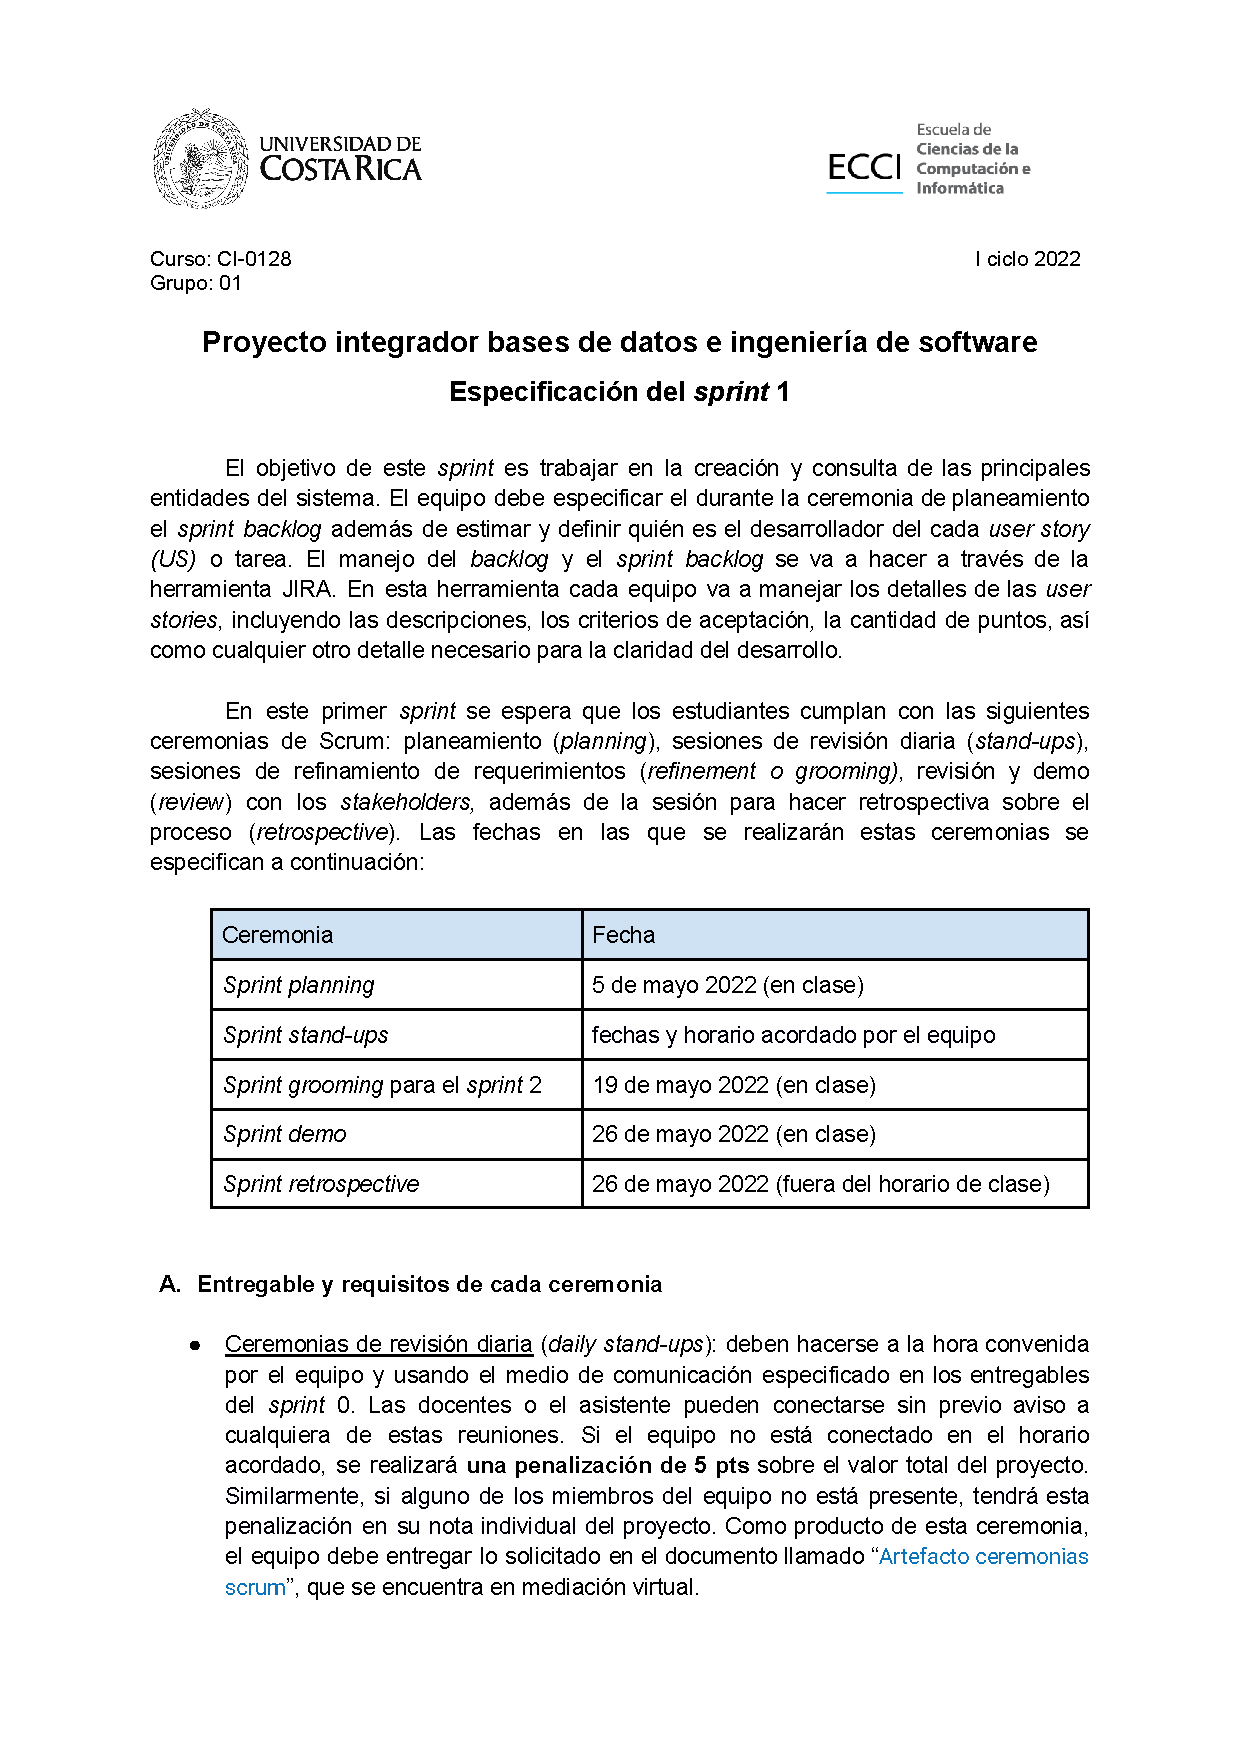
\includepdf[pages={-}]{../enunciado_sprint1.pdf}

\newpage
\section{Código fuente del Git}
El enlace del repositorio es el siguiente: \url{https://github.com/emasp2001/pi_ingeBases/tree/main/Planilla};
dado que este es un repositorio privado la invitación a la profesora había sido enviada,
sin embargo esta no fue aceptada dentro del tiempo rango establecido por Github 
por lo que automaticamente expiró, por lo que se le vuelve a enviar el día
26 de mayo a la 1:00am. El asistente (usuario: \textit{ChristianRojasRios}) ya había aceptado la invitación por lo que él 
sí se encuentra dentro del repositorio.\\
Cabe mencionar que se siguió la regla de completar las user stories por medio de
diferentes \textit{branch} y \textit{pull requests}.

\section{Sprint backlog de Jira}
El enlace donde se encuentra el \textit{sprint backlog} es el siguiente: \url{https://ingesoftg001.atlassian.net/jira/software/projects/TB/boards/5/backlog}.

\section{Entregable de las ceremonias Scrum}
Se encuentra adjunto en el archivo \textbf{bitacora\_ceremonias.pdf}.

\section{Mock ups de la aplicación}
Los Mock Ups de esta aplicación han sido aprobados por el \textit{Project Owner} y se
encuentran disponibles en esta carpeta de este entregable bajo el nombre de \textbf{\textit{mock\_ups.pdf}}.

\section{Diagrama de clases - UML}
El diagrama de clases UML de este proyecto se encuentra adjunto en esta carpeta de
entrega bajo el nombre \textbf{\textit{diagrama\_uml.pdf}}.

\section{Diseño lógio de la base de datos e implementación}
\subsection{Modelo Lógico Relacional}
Estos se encuentran adjuntos en esta carpeta de entrega bajo el nombre de
\textbf{\textit{modelo\_logico\_database.pdf}} para el modelo lógico relacional de tablas,
y bajo el nombre \textbf{\textit{modelo\_entidad\_relacion.pdf}} para el modelo
de entidad \- relación.

\subsection{Script SQL}
Este script se encuentra también adjunto en esta carpeta bajo el nombre
\textbf{\textit{TaBueno\_Query.sql}}, sin embargo a modo de \textbf{respaldo}
se adjunta también ese mismo código en este archivo:
\begin{minted}{sql}
------------------------- Oficial Ta' Bueno SQL Query -------------------------
use TaBueno

--------------- Creating Tables --------------
-- Entidad: Usuario
create table Usuario 
    (Cedula         char(10)        NOT NULL, 
    Contrasena      varchar(50)     NOT NULL,
    Nombre          varchar(15)     NOT NULL,
    Apellido1       varchar(15)     NOT NULL,
    Apellido2       varchar(15)     NOT NULL,
    Telefono        int             NOT NULL,
    TipoUsuario     tinyint         NOT NULL,
    Provincia       varchar(15)     NOT NULL,
    Canton          varchar(15)     NOT NULL,
    CodigoPostal    char(5)         NOT NULL,
    primary key (Cedula)
);

-- Entidad: Proyecto
create table Proyecto
    (nombre             varchar(200)        not null,
    cedulaEmpleador     char(10)            not null,
    presupuesto         float,
    modalidadPago       varchar(50),
    primary key (nombre, cedulaEmpleador),
    foreign key (cedulaEmpleador) references Usuario
);

-- Entidad: Deducciones Obligatorias
create table DeduccionesObligatorias
    (nombre             varchar(100)        not null,
    porcentaje          float       
    primary key (nombre)
);

-- Relacion: TrabajaEn
create table TrabajaEn
    (nombreProyecto         varchar(200)        not null,
    cedulaEmpleador         char(10)            not null,
    cedulaEmpleado          char(10)            not null,
    registroHoras           INT,
    primary key (nombreProyecto, cedulaEmpleador, cedulaEmpleado),
    foreign key (nombreProyecto, cedulaEmpleador) references Proyecto
);

-- Entidad: Beneficios
create table Beneficios
    (nombreBeneficio        varchar(200)        not null,
    cedulaEmpleador         char(10)            not null,
    nombreProyecto          varchar(200)        not null,
    primary key (nombreBeneficio, cedulaEmpleador, nombreProyecto),
    foreign key (nombreProyecto, cedulaEmpleador) references Proyecto
);

-- Entidad: Pago
create table Pago
    (cedulaRecibe           char(10)            not null,
    fecha                   date                not null,
    nombreProyecto          varchar(200)        not null,
    cedulaEmpleador         char(10)            not null,
    salarioBruto            float,
    tipoPago                varchar(50),
    primary key (cedulaRecibe, fecha),
    foreign key (nombreProyecto, cedulaEmpleador) references Proyecto
);

-- Relacion: IncluyeDeduccionObligatoria
create table IncluyeDeduccionObligatoria
    (cedulaEmpleado                 char(10)            not null,
    fechaPago                       date                not null,
    nombreDeduccionObligatoria      varchar(100)        not null,
    primary key (cedulaEmpleado, fechaPago, nombreDeduccionObligatoria),
    foreign key (cedulaEmpleado, fechaPago) references Pago,
    foreign key (nombreDeduccionObligatoria) references DeduccionesObligatorias
);

-- Entidad: Contrato
create table Contrato
    (nombreProyecto         varchar(200)        not null,
    cedulaEmpleador         char(10)            not null,
    cedulaEmpleado          char(10)            not null,
    fechaInicio             date                not null,
    puesto                  varchar(100)        not null,
    fechaFinalizacion       date,
    jornadaLaboral          varchar(200),
    primary key (nombreProyecto, cedulaEmpleador, cedulaEmpleado, fechaInicio),
    foreign key (nombreProyecto, cedulaEmpleador) references Proyecto,
    foreign key (cedulaEmpleado) references Usuario
);

-- Entidad: EstadoBeneficio
create table EstadoBeneficio
    (nombreBeneficio        varchar(200)        not null,
    cedulaEmpleador         char(10)            not null,
    nombreProyecto          varchar(200)        not null,
    fechaInicio             date,
    fechaFinalizacion       date,
    primary key (nombreBeneficio, cedulaEmpleador, nombreProyecto, fechaInicio),
    foreign key (nombreBeneficio, cedulaEmpleador, nombreProyecto) references Beneficios
);

-- Relacion: ApareceEn
create table ApareceEn
    (nombreBeneficio        varchar(200)        not null,
    cedulaEmpleador         char(10)            not null,
    nombreProyecto          varchar(200)        not null,
    fechaInicio             date,
    cedulaRecibePago        char(10),
    fechaPago               date,
    primary key (nombreBeneficio, cedulaEmpleador, nombreProyecto, fechaInicio,
                cedulaRecibePago, fechaPago),
    foreign key (nombreBeneficio, cedulaEmpleador, nombreProyecto, fechaInicio)
    references EstadoBeneficio
);

-- Entidad: DeduccionesVoluntarias
create table DeduccionesVoluntarias
    (nombre                 varchar(100)        not null,
    primary key (nombre)
);

-- Entidad: EstadoDeduccionVoluntaria
create table EstadoDeduccionVoluntaria
    (nombreDeduccion        varchar(100)        not null,
    fechaInicial            date                not null,
    fechaFinalizacion       date,
    monto                   float               not null,
    nombreProyecto          varchar(200)        not null,
    cedulaEmpleador         char(10)            not null,
    primary key (nombreDeduccion, fechaInicial),
    foreign key (nombreProyecto, cedulaEmpleador) references Proyecto
);

-- Relacion: IncluyeDeduccionVoluntaria
create table IncluyeDeduccionVoluntaria
    (nombreDeduccion        varchar(100)        not null,
    fechaInicialDeduccion   date                not null,
    fechaPago               date                not null,
    cedulaRecibePago        char(10)            not null,
    primary key (nombreDeduccion, fechaInicialDeduccion, fechaPago, cedulaRecibePago),
    foreign key (nombreDeduccion, fechaInicialDeduccion) references EstadoDeduccionVoluntaria,
    foreign key (cedulaRecibePago, fechaPago) references Pago
);


--------------- Inserting Values --------------
-- Usuarios
insert into Usuario values ('1234567890', 'password', 'Diego', 'Chinchilla', 'Otarola',
                            '76343352', 0, 'San Jose', 'Hatillo', '10101');
insert into Usuario values ('0987654321', 'password', 'Jan', 'Murillo', 'Barquero',
                            '23213433', 1, 'Alajuela', 'Alajuela', '20201');
insert into Usuario values ('2365123132', 'password', 'Gabriel', 'Zuniga', 'Orozco',
                            '35435344', 1, 'Heredia', 'Heredia', '30301');

-- Proyectos
insert into Proyecto values ('Sistema de Planilla CR', '1234567890', '0987654321', 0)

-- Deducciones Obligatorias
insert into DeduccionesObligatorias values ('Caja Costarricense de Seguro Social', 0.10);
insert into DeduccionesObligatorias values ('Impuesto al Valor Agregado', 0.05);
Insert into DeduccionesObligatorias Values ('Enfermedad y Maternidad', 0.055)
Insert into DeduccionesObligatorias Values ('Invalidez, Vejez y Muerte', 0.0384)
Insert into DeduccionesObligatorias Values ('Aporte Trabajador', 0.1)
Insert into DeduccionesObligatorias Values ('Bajo 863000', 0)
Insert into DeduccionesObligatorias Values ('Hasta 1267000', 0.1)
Insert into DeduccionesObligatorias Values ('Hasta 2223000', 0.15)
Insert into DeduccionesObligatorias Values ('Hasta 4445000', 0.20)
Insert into DeduccionesObligatorias Values ('Sobre 4445000', 0.25)

-- Beneficios
insert into Beneficios values ('Plan Dental', '1234567890', 'Sistema de Planilla CR')

--------------- Consulting Values --------------
select * from Usuario
select * from Proyecto
select * from Beneficios
select * from DeduccionesObligatorias

\end{minted}


\section{Presentación durante el \textit{sprint review}}
Se realizó la presentación de este código el día 26 de Mayo del 2022.

\section{Autoevaluación y coevaluación}
Cada miembro del equipo debió ser responsable de adjuntar su propia autoevaluación
y coevaluación.

%\begin{figure}[h]
%  \centering
%  \includegraphics[width=0.65\textwidth]{SystemCalls.png}
%  \caption{Funcionamiento interno de una interrupción al Sistema Operativo \cite[]{whatSysCalls}.}
%  \label{fig:HowWorksSysCalls}
%\end{figure}

%---------------------- Document Ending ----------------------------------
%\newpage
%\bibliographystyle{apacite}
%\bibliography{bibliography.bib}
\end{document}
